
\section{Ergebnisse}

In diesem Kapitel werden die Ergebnisse der einzelnen Zwischenschritte der Methodik nach \autoref{chap:Methodik} dargestellt und kritisch betrachtet.
Hierzu gehören vorerst die Ergebnisse der Clusterung der \gls{MS}-Netzgebiete, die mit \gls{SIMBEV} erzeugten Fahrtprofile und Standzeiten von \gls{EPKW} und deren räumlicher Verteilung, sowie die Ergebnisse der Implementierung der verschiedenen Ladestrategien.
Abschließend erfolgt eine detaillierte Betrachtung der Ergebnisse der Ermittlung des Abregelungsbedarfes aufgrund der Integration von \glspl{EPKW} für die untersuchten Netze.


\subsection{Clusterung der MS-Netzgebiete}

Auf der \gls{MS}-Ebene gibt es \num{3591} Netzgebiete mit einer mittleren Fläche von \SI{99}{\km\squared}.
Die vollständige Untersuchung der mit Hilfe des Open Source Tools \gls{DINGO} synthetisierten \gls{MS}-Netzgebiete, würde aufgrund ihrer großen Anzahl zu inakzeptabel hohen Rechenzeiten führen.
Im Rahmen dieser Masterarbeit wurden sechs Referenznetzgebiete ausgewählt, welche \num{1842} der \num{3591} {\color{red} TODO 3354?} \gls{MS}-Netzgebiete repräsentieren.
Das Clustering erfolgte innerhalb \cite{Schachler} durch den während des \openego Projektes entwickelten k-means-Clusteralgorithmus nach \autoref{chap:dingo_theo}.

\begin{figure}[H]
    \centering
    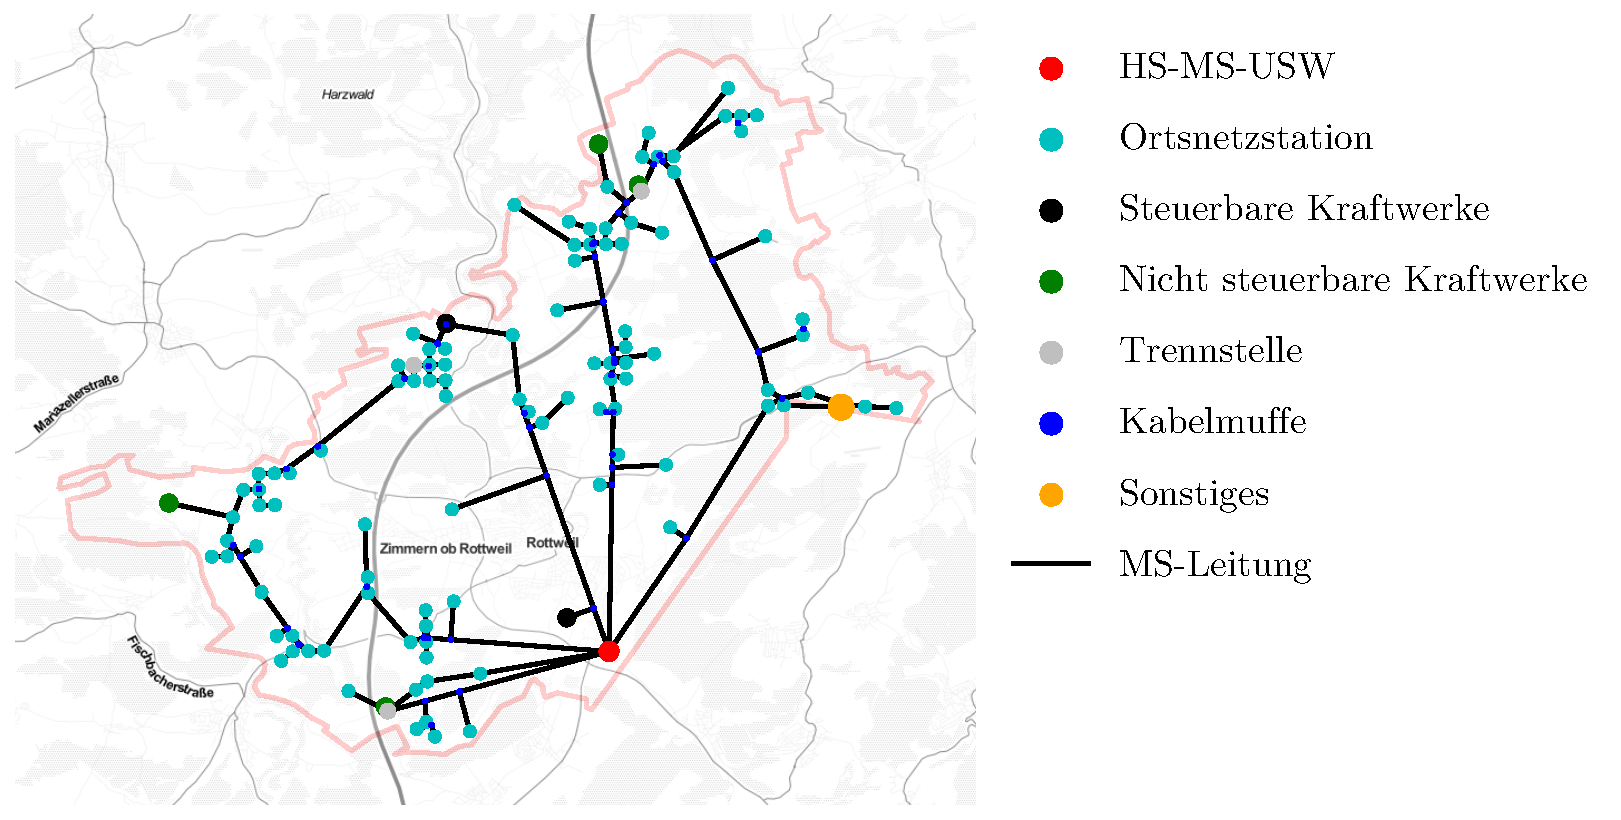
\includegraphics[width=\textwidth]{Bilder/grid_176_map}
    \caption{Beispielhafte Darstellung des MS-Netzes \num{176} mit allen Umspannwerken, Erzeugerkapazitäten und sonstigen Betriebsmitteln}\label{fig:grid_176_map}
\end{figure}

\autoref{fig:grid_176_map} zeigt den Aufbau eines beispielhaften Mittelspannungsnetzes, welches mit Hilfe von \gls{DINGO} erzeugt wurde und innerhalb dieser Arbeit untersucht wurde.
Um mit dieser Arbeit eine Ergänzung zu \cite{Schachler} zu liefern, wird das Clustering \cite{Schachler} übernommen und von den \num{15} identifizierten repräsentativen Netzgebieten eine Teilmenge untersucht.
So werden jeweils zwei Netzgebiete der Kategorien Wind-, \gls{PV}- und Last-dominiert ausgewählt, die möglichst viele Netzgebiete repräsentieren.
Auf diese Weise wird sichergestellt, dass die Effekte der Netzintegration der Elektromobilität auf möglichst unterschiedliche Netze aufgezeigt werden können.
Insgesamt werden somit sechs Netzgebiete untersucht, die stellvertretend für \num{1842} der \num{3591} Mittelspannungsnetze stehen.
In \autoref{tab:grid_IDs} finden sich die \glspl{ID} der untersuchten Mittelspannungsnetze und die Anzahl an repräsentierten Netzgebieten.

{
\renewcommand{\arraystretch}{1.2}% grßerer Zeilenabstand
\sisetup{range-phrase=~{--}~}% Gedankenstrich statt "bis" bei SIrange
\begin{table}[H]
	\begin{center}
		\caption{Anzahl der repräsentierten Netzgebiete und Kategorie der untersuchte Mittelspannungsnetze}
		\begin{tabu} to \textwidth {X[1] X[1] X[1, r] }
			\hline
			Netz ID    & Kategorie      & Anzahl repräsentierter Netze \\ \hline
			\num{176}  & PV-dominiert   & \num{413}                    \\
			\num{177}  & Last-dominiert & \num{666}                    \\
			\num{1056} & PV-dominiert   & \num{197}                    \\
			\num{1690} & Wind-dominiert & \num{141}                    \\
			\num{1811} & Wind-dominiert & \num{78}                     \\
			\num{2534} & Last-dominiert & \num{347}                    \\ \hline
		\end{tabu}
		\label{tab:grid_IDs}
	\end{center}
	\vspace{-3mm}%Put here to reduce too much white space after your table
\end{table}
}

In \autoref{fig:bar_representatives} findet sich eine Darstellung der wichtigsten Charakteristika der untersuchten Netzgebiete.
Hierzu zählen die installierten \gls{PV}- und Wind-Kapazitäten, sowie die Spitzenlast der \glspl{EPKW} bei einem ungesteuerten Laden im Antriebswende-Szenario und die Spitzenlast des konventionellen Stromverbrauchs inklusive \glspl{WP}.
Weiterhin findet sich in \autoref{fig:map_representatives} eine Karte der repräsentierten Netzgebiete eingeteilt in die Kategorien Wind-, \gls{PV}- und Last-dominiert.

\begin{figure}[H]
    \centering
    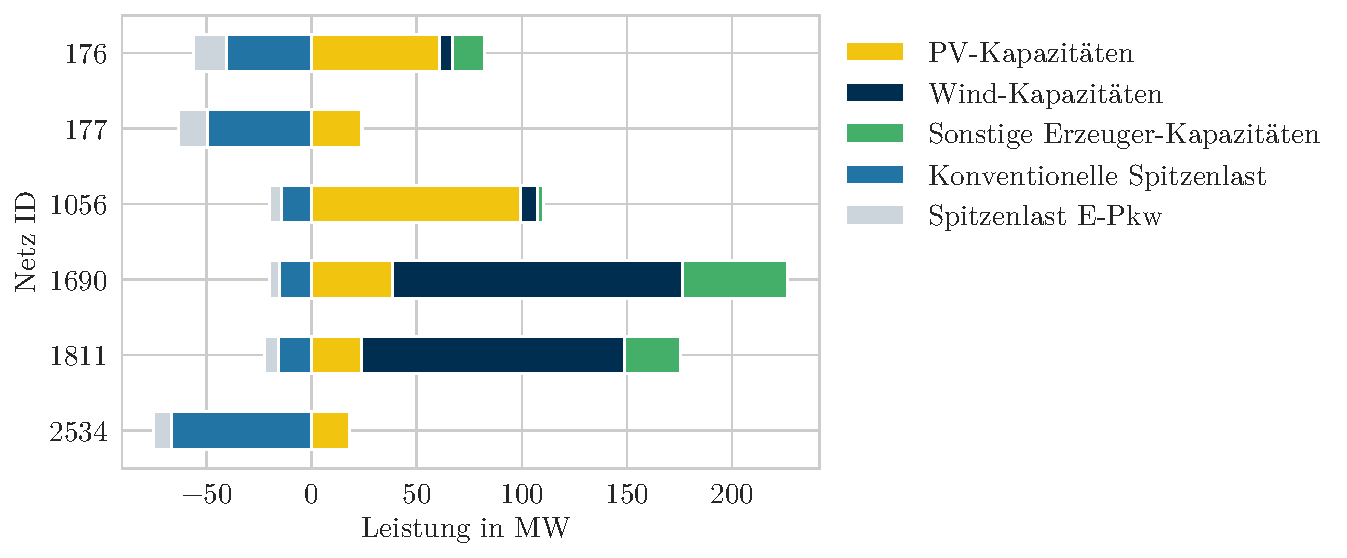
\includegraphics[width=\textwidth]{Bilder/Installed_cap_peak_load_representatives}
    \caption{Kumulierte Wirkleistung von PV-, Wind- und sonstigen Erzeuger-Kapazitäten sowie die kumulierte konventionelle und mobilitätsbedingte Spitzenlast in den Referenznetzgebieten}\label{fig:bar_representatives}
\end{figure}

\begin{figure}
    \centering
    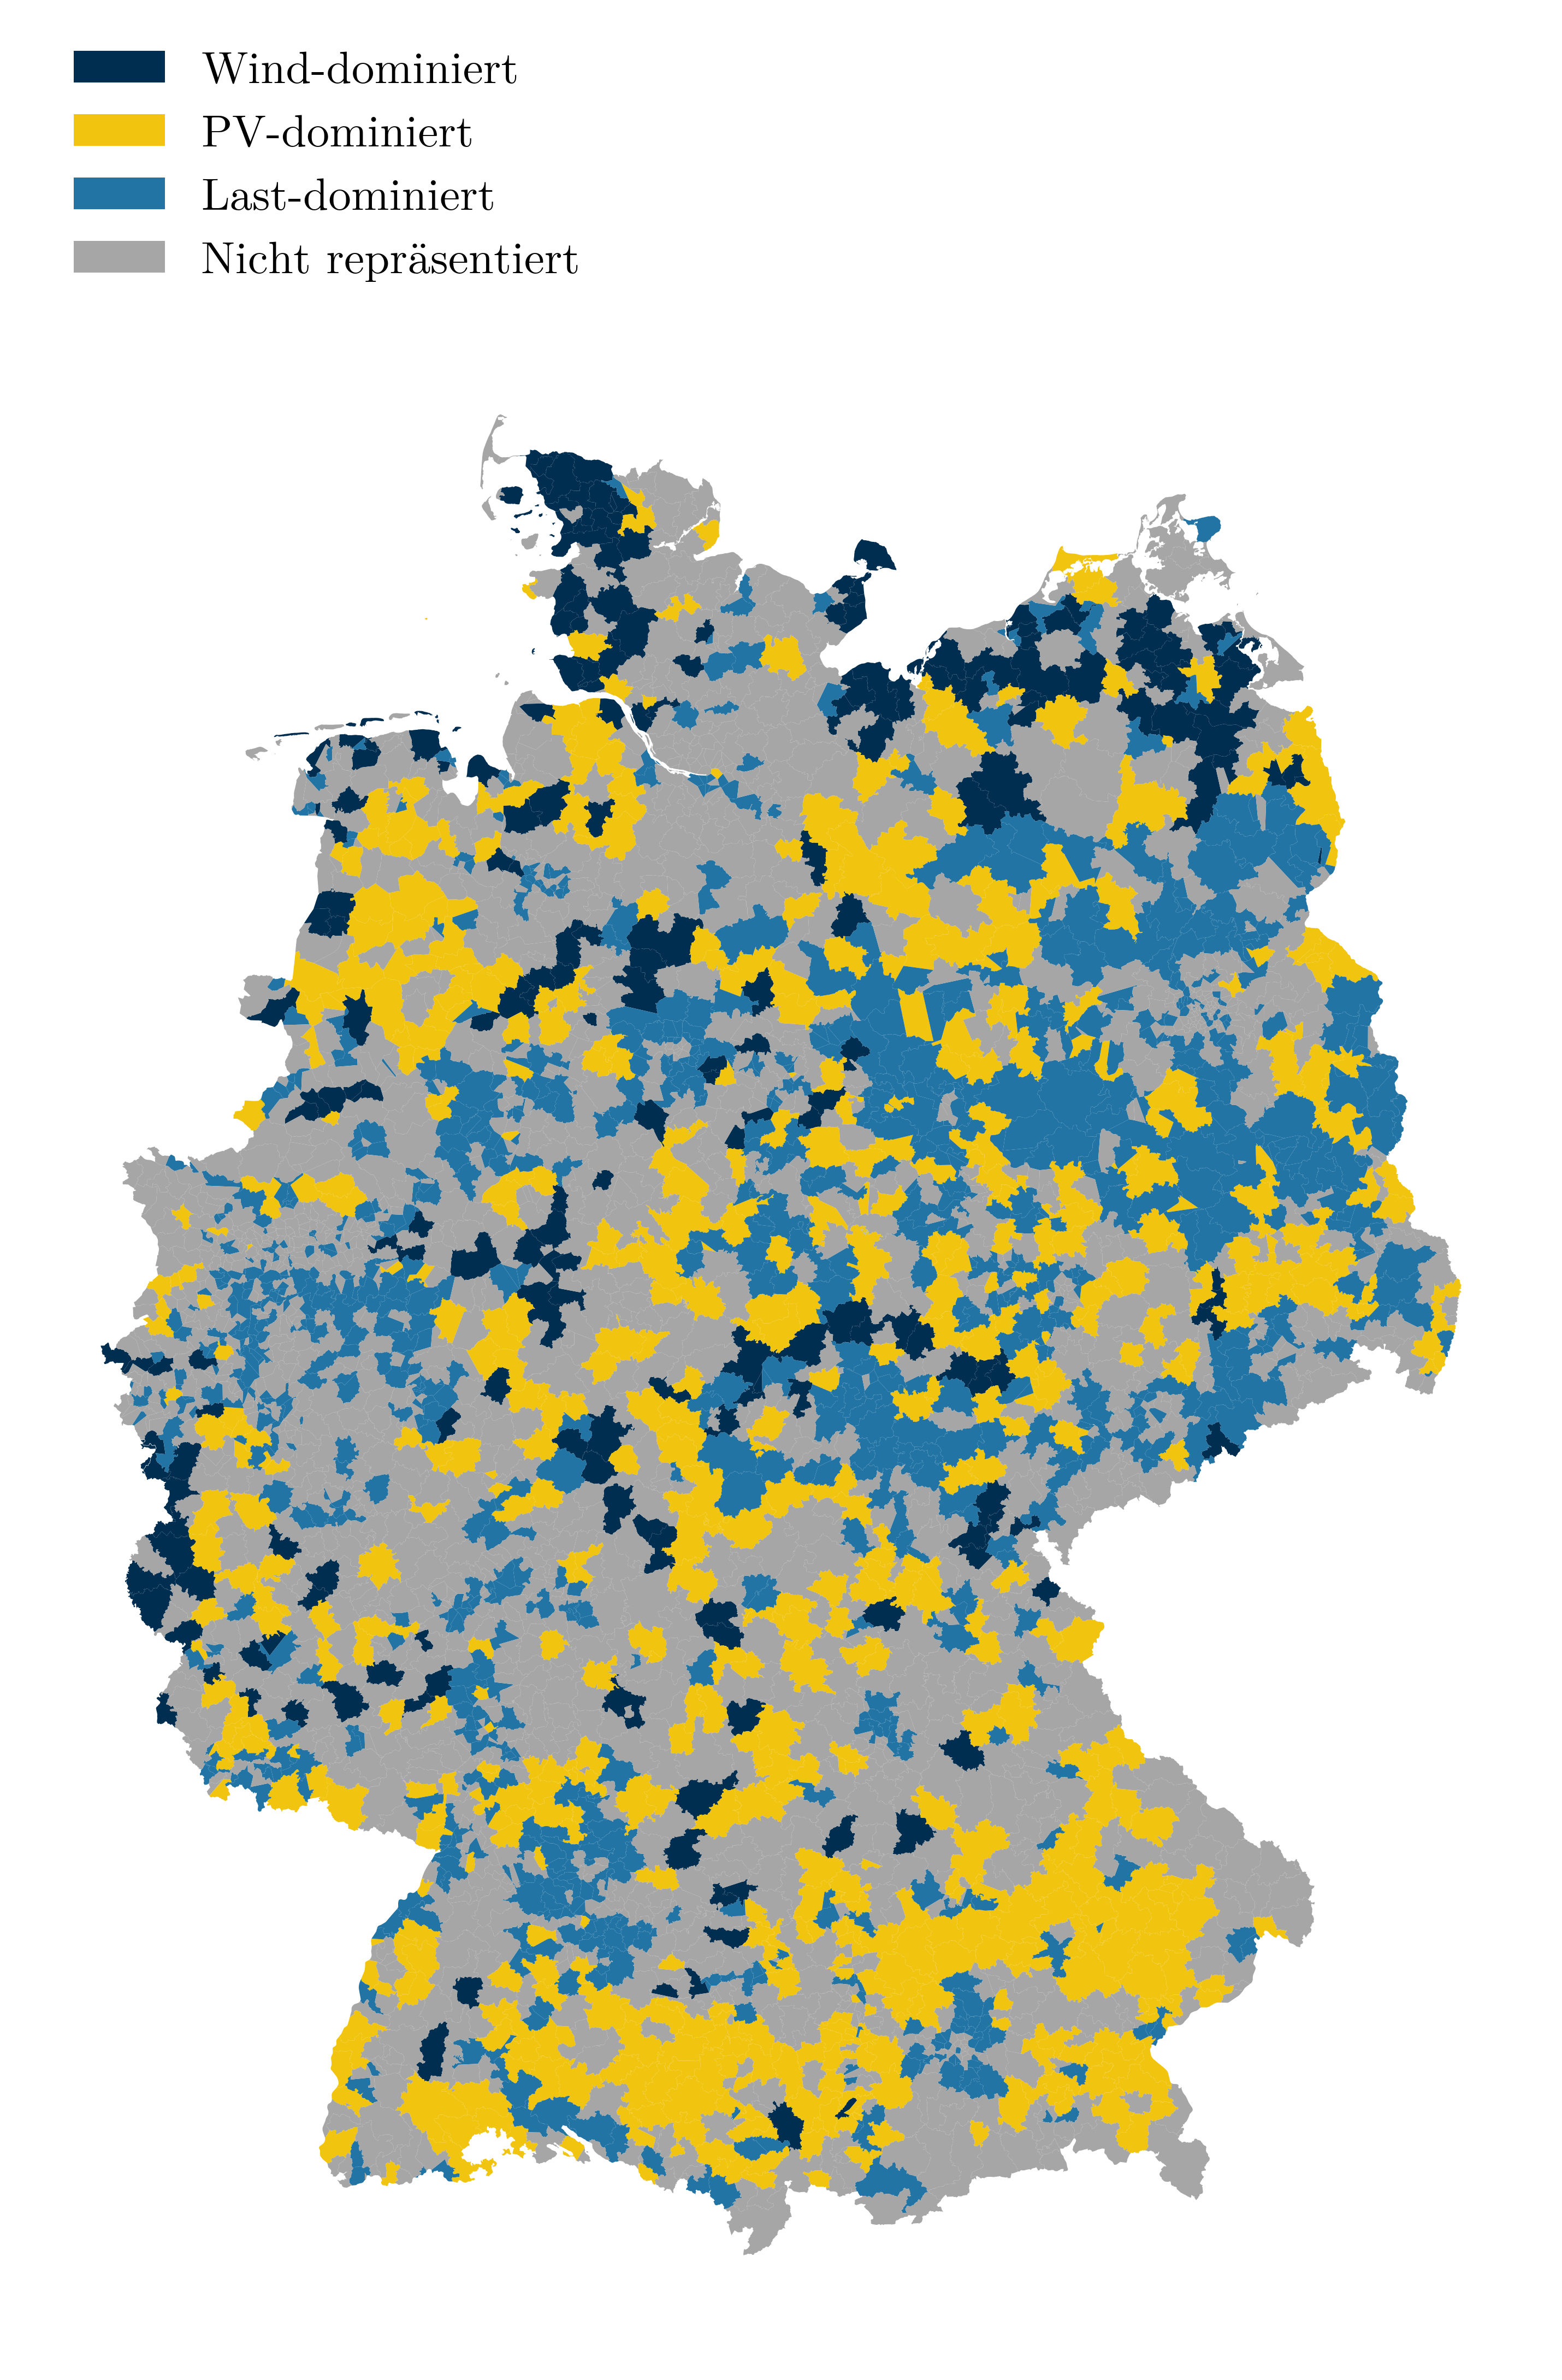
\includegraphics[width=\textwidth]{Bilder/clusters_representatives}
    \caption{Repräsentierte Netzgebiete in Deutschland}\label{fig:map_representatives}
\end{figure}


\subsection{Erzeugung und Charakteristik der Fahrtprofile}

Mit Hilfe des Software Tools \gls{SIMBEV} können für die zuvor geclusterten Referenznetzgebiet die Fahrtprofile der im Netzgebiet befindlichen Fahrzeuge erzeugt werden.
Die Charakteristik der Fahrtprofile spielt eine entscheidende Rolle für die Wirksamkeit der unterschiedlichen Ladestrategien und die Auswirkungen auf die Netze.
Hierbei steht vor allem die Jahresfahrleistung der \glspl{EPKW} und der Anteil flexibilisierbarer und nicht-flexibilisierer Ladevorgänge im Vordergrund.\medskip

Die Ermittlung der Anzahl der Fahrzeuge erfolgt nach \autoref{chap:simbev_theo} auf Gemeindeebene.
In der Regel liegen innerhalb eines Netzgebietes mehrere Gemeinden und insgesamt liegen \num{35} Gemeinden innerhalb der sechs Referenznetzgebiete.
Die Auswertung ergibt die Anzahl der simulierten Fahrzeuge nach \autoref{tab:car_count} je Fahrzeugtyp und Szenario.
Zusätzlich findet sich im Anhang in \autoref{tab:car_count_long} eine detailliertere Aufteilung je Fahrzeugtyp, -klasse und Szenario.

{
\renewcommand{\arraystretch}{1.2}% grßerer Zeilenabstand
\sisetup{range-phrase=~{--}~}% Gedankenstrich statt "bis" bei SIrange
\begin{table}[H]
	\begin{center}
		\caption{Anzahl der simulierten Fahrzeuge je Typ und Szenario}
		\begin{tabu} to 0.6\textwidth {X[1.2] X[1, r] X[1, r] X[1, r]}
			\hline
			Szenario         & BEV         & PHEV        & Summe       \\ \hline
			NEP C \num{2035} & \num{16598} & \num{10283} & \num{26881} \\
			Referenz         & \num{29712} & \num{18407} & \num{48119} \\
			Mobilitätswende  & \num{44750} & \num{27726} & \num{72476} \\
			Kleinwagen       & \num{54355} & \num{18121} & \num{72476} \\
			Antriebswende    & \num{56547} & \num{35029} & \num{91576} \\ \hline
		\end{tabu}
		\label{tab:car_count}
	\end{center}
	\vspace{-3mm}%Put here to reduce too much white space after your table
\end{table}
}

Die \num{35} Gemeinden weisen drei der sieben \gls{REGIOSTAR} (s. \autoref{tab:RegioStaR}) auf.
Hierzu zählen der kleinstädtische, dörfliche Raum einer ländlichen Region (\gls{ID} \num{77}), Mittelstädte, städitscher Raum (\gls{ID} \num{76}) und Mittelstädte, städitscher Raum einer Stadtregion (\gls{ID} \num{73}).
Eine Analyse der erzeugten Fahrtprofile zeigt, dass in \gls{ID} \num{77} im Schnitt die weitesten Strecken zurückgelegt werden, welches den Erwartungen nach \gls{MID} \cite{Nobis2019} entspricht.
Jedoch liegen die Jahresfahrleistungen insgesamt unter den Angaben des \gls{MID} von durchschnittlich \SI{14700}{\km}, aber auf einem ähnlichen Niveau zu einer Auswertung von Kfz-Versicherungen des Vergleichsportals \textit{Check24} \cite{CHECK24GmbH2018}, wonach die durchschnittliche Jahresfahrleistung in Deutschland im Jahr \num{2017} bei \SI{11888}{\km} lag.
Insgesamt spiegeln die Jahresfahrleistungen \glspl{SIMBEV} somit ein progressives Szenario mit einer sinkenden Jahresfahrleistung wider.
Die Jahresfahrleistung von \glspl{BEV} je \gls{REGIOSTAR} \gls{ID} wurde zusammenfassend über alle Szenarien hinweg berechnet und findet sich in \autoref{tab:bev_distance}.

{
\renewcommand{\arraystretch}{1.2}% grßerer Zeilenabstand
\sisetup{range-phrase=~{--}~}% Gedankenstrich statt "bis" bei SIrange
\begin{table}[H]
	\begin{center}
		\caption{Durchschnittliche und maximale Jahresfahrleistung von BEVs je untersuchter Raumtypologie}
		\begin{tabu} to \textwidth {X[1] X[1.5, r] X[1.5, r]}
			\hline
			Raumtypologie ID 	   & Durchschnittle Jahresfahrleistung                  & Maximale Jahresfahrleistung \\ \hline
			\num{77}               & \SI[separate-uncertainty = true]{12353(6395)}{\km} & \SI{55.426}{\km}            \\
			\num{76}               & \SI[separate-uncertainty = true]{11500(6243)}{\km} & \SI{54.204}{\km}            \\
			\num{73}               & \SI[separate-uncertainty = true]{11660(6408)}{\km} & \SI{58.575}{\km}            \\ \hline
		\end{tabu}
		\label{tab:bev_distance}
	\end{center}
	\vspace{-3mm}%Put here to reduce too much white space after your table
\end{table}
}

Eine Betrachtung der durchschnittlichen Stand- und Ladezeiten bei maximal möglicher Ladeleistung der \gls{EPKW} je Wegezweck (s. \autoref{tab:StandingTime}) zeigt, dass die \gls{EPKW} vor allem im privaten Bereich einen Großteil der Standzeit nicht geladen werden.
So macht die durchschnittliche Ladezeit zu Hause oder am Arbeitsplatz nur etwa \SI{8}{\percent} der Standzeit aus.
Dies zeigt deutlich das große Flexibilisierungspotential im privaten Bereich.
Allerdings fällt auf, dass die mit \gls{SIMBEV} ermittelten Standzeiten im öffentlichen Bereich unrealistisch lang erscheinen.

{
\renewcommand{\arraystretch}{1.2}% grßerer Zeilenabstand
\sisetup{range-phrase=~{--}~}% Gedankenstrich statt "bis" bei SIrange
\begin{table}[H]
	\begin{center}
		\caption{Durchschnittliche Stand- und Ladezeiten je Wegezweck}
		\begin{tabu} to 0.8\textwidth {X[0.5] X[1, r] X[1, r]}
			\hline
			Wegezweck  & Durchschnittliche Standzeit                      & Durchschnittliche Ladezeit	                     \\ \hline
			Arbeit     & \SI[separate-uncertainty = true]{7.3(37)}{\hour} & \SI[separate-uncertainty = true]{0.6(5)}{\hour}  \\
			dienstlich & \SI[separate-uncertainty = true]{4.4(58)}{\hour} & \SI[separate-uncertainty = true]{1.1(7)}{\hour}  \\
			Ausbildung & \SI[separate-uncertainty = true]{6.2(39)}{\hour} & \SI[separate-uncertainty = true]{1.4(11)}{\hour} \\
			Einkauf    & \SI[separate-uncertainty = true]{2.1(38)}{\hour} & \SI[separate-uncertainty = true]{0.8(5)}{\hour}  \\
			Erledigung & \SI[separate-uncertainty = true]{4.2(56)}{\hour} & \SI[separate-uncertainty = true]{0.9(6)}{\hour}  \\
			Freizeit   & \SI[separate-uncertainty = true]{6.0(62)}{\hour} & \SI[separate-uncertainty = true]{1.1(7)}{\hour}  \\
			nach Hause & \SI[separate-uncertainty = true]{8.9(57)}{\hour} & \SI[separate-uncertainty = true]{0.7(6)}{\hour}  \\ \hline
		\end{tabu}
		\label{tab:StandingTime}
	\end{center}
	\vspace{-3mm}%Put here to reduce too much white space after your table
\end{table}
}

Der Anteil flexibilisierbarer Ladevorgänge entspricht dem Anteil an Energie am Gesamtenergiebedarf der \glspl{EPKW}, der an privaten Ladepunkten zu Hause oder am Arbeitsplatz nachgeladen wird.
Hierzu zählen alle Ladevorgänge die am Eigenheim, einer Wohnaalage oder auf einem Firmenparkplatz stattfinden.
Zusätzlich sind nur Ladevorgänge flexibilisierbar, deren Standzeit größer ist als die Mindestladedauer.
Demgegenüber stehen nicht-flexibilisierer Ladevorgänge im öffentlichen Raum und an Schnellladestationen bzw. Ladevorgänge deren Standzeit der Mindestladedauer entspricht.
Im Mittel liegt der Anteil flexibilisierer Ladevorgänge über alle Szenarien je Gemeinde bei \SI{71.1}{\percent}.
Hiervon ausgenommen ist die \SzeFirmenparkplatzdot, bei der es aufgrund des geringeren Bestands an Ladeinfrastruktur am Arbeitsplatz zu mehr Ladevorgängen im öffentlichen Raum kommt.
Der Anteil flexibilisierer Ladevorgänge liegt bei dieser Szenarette bei \SI{66.1}{\percent}.
In \autoref{tab:ChargingShare} sind die Anteile in flexibilisierbare und nicht-flexibilisierbare Ladevorgänge zusammengefasst.

{
\renewcommand{\arraystretch}{1.2}% grßerer Zeilenabstand
\sisetup{range-phrase=~{--}~}% Gedankenstrich statt "bis" bei SIrange
\begin{table}[H]
	\begin{center}
		\caption{Aufteilung in flexibiliserbare und nicht-flexibiliserbare Ladevorgänge}
		\begin{tabu} to \textwidth {X[1] X[1, r] X[1, r]}
			\hline
								  					& \SzeFirmenparkplatzdot                               & Sonstige Szenarien                                   \\ \hline
			Flexibiliserbar$^{\mathrm{a}}$       	& \SI[separate-uncertainty = true]{66.1(23)}{\percent} & \SI[separate-uncertainty = true]{71.1(23)}{\percent} \\
			Nicht-flexibiliserbar$^{\mathrm{a}}$ 	& \SI[separate-uncertainty = true]{33.9(23)}{\percent} & \SI[separate-uncertainty = true]{28.9(23)}{\percent} \\ \hline
			\multicolumn{3}{l}{$^{\mathrm{a}}$Anteil vom Gesamtenergiebedarf der E-Pkw je Gemeinde mit Standardabweichung}
		\end{tabu}
		\label{tab:ChargingShare}
	\end{center}
	\vspace{-3mm}%Put here to reduce too much white space after your table
\end{table}
}

In \autoref{fig:example_load_profile} findet sich ein beispielhaftes \gls{EPKW}-Lastprofil für ungesteuertes Laden einer mittelstädtischen Gemeinde (\gls{ID} \num{73}) mit \num{6443} \glspl{EPKW} über eine Woche im Antriebswende-Szenario (links).
Zusätzlich ist das \gls{EPKW}-Lastprofil der gleichen Gemeinde in der \SzeFirmenparkplatz (rechts) dargestellt.

\begin{figure}[H]
    \centering
    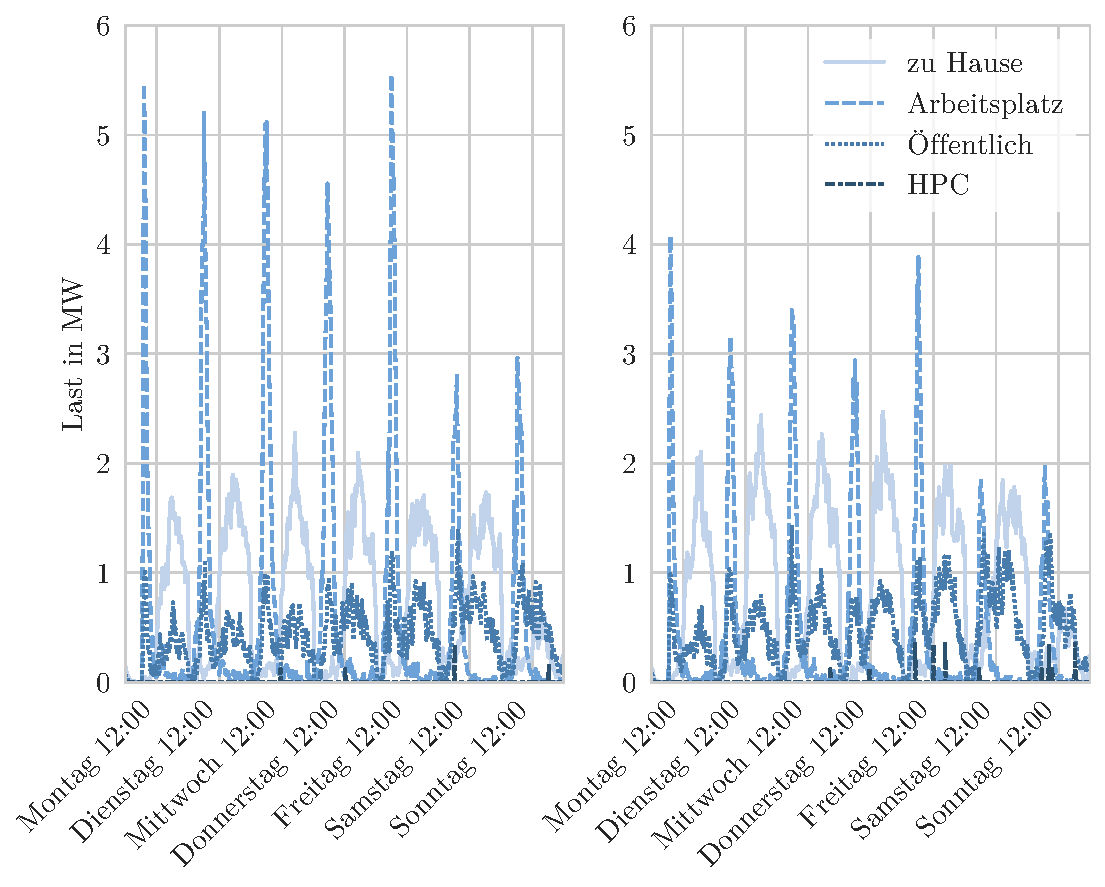
\includegraphics[width=\textwidth]{Bilder/example_load_profile}
    \caption{E-Pkw-Lastprofil für ungesteuertes Laden einer mittelstädtischen Gemeinde mit \num{6443} E-Pkws über eine Woche im Elektrifizierungs-Szenario (links) und der \SzeFirmenparkplatz (rechts)}\label{fig:example_load_profile}
\end{figure}

Die Lastgänge \zH und \Firmeparkplatz entsprechen den Ladevorgängen im privaten Bereich.
Unter dem Lastgang \oeffen sind hingegen alle öffentlichen Ladevorgänge mit Außnahme der Schnellladevorgänge (\gls{HPC}) zusammengefasst.
Deutlich zu erkennen ist die hohe Gleichzeitigkeit am Vormittag sowohl am \Firmeparkplatz als auch im öffentlichen Raum, welche durch das Fahren zur Arbeit ausgelöst wird.
Auch die Rückkehr zum Wohnort ist ab dem frühen Nachmittag in den Lastgängen \zH und im öffentlichen Raum deutlich zu erkennen. Die entsprechenden Dauerlastkurven für die Gemeinde über eine Woche (s. \autoref{fig:example_load_curve}) zeigen dies nochmals deutlich.
Schnellladevorgänge treten unregelmäßig im Verlauf der Woche auf.
Am Wochenende kommt es zu deutlich geringeren Anteilen von Ladevorgängen \zH und am \Firmeparkplatzdot, wodurch das Flexibilisierungspotential am Wochenende geringer ausfällt.
Gegenüber dem Antriebswende-Szenario sinkt die Höchstlast in der \SzeFirmenparkplatzdot.
Jedoch sinkt auch das Flexibilisierungspotential bei gleichbleibendem Energiebedarf durch die Verschiebung der Ladevorgänge in den öffentlichen Raum.

\begin{figure}[H]
    \centering
    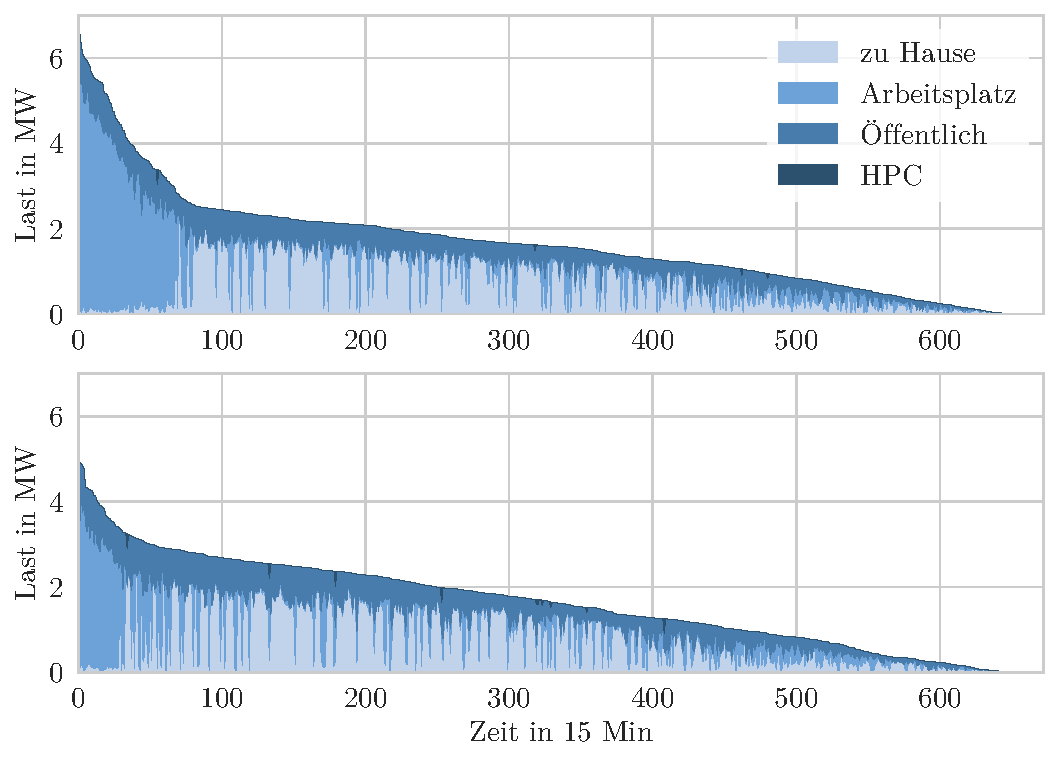
\includegraphics[width=\textwidth]{Bilder/example_load_duration_curve}
    \caption{E-Pkw-Dauerlastkurve für ungesteuertes Laden einer mittelstädtischen Gemeinde mit \num{6443} E-Pkws über eine Woche im Elektrifizierungs-Szenario (oben) und der \SzeFirmenparkplatz (unten)}\label{fig:example_load_curve}
\end{figure}


\subsubsection{Kritik}

Die erstellten Fahrtprofile spiegeln ein plausibel erscheinendes Bild wider.
Dennoch existieren einzelne Kritikpunkte, die innerhalb des \gls{SIMBEV} Projektes gelöst werden sollten.
So ist es zum Zeitpunkt der Erstellung der Fahrtprofile noch nicht möglich, einen längeren Zeitraum als eine Woche am Stück zu simulieren.
Da sich jedoch die Netzuntersuchungen im Rahmen dieser Masterarbeit auf einen Zeitraum von zwei Wochen beziehen, wird die simulierte Woche stellvertretend für beide Wochen verwendet.
Hierfür wurde jedes Fahrtprofil eines \gls{EPKW} solange mit sich selbst verlängert und logisch verknüpft, bis die gewünschte Länge erreicht wurde.
Dieses Vorgehen bringt jedoch einige Nachteile mit sich.
Durch den kurzen simulierten Zeitraum fällt der \gls{SOC} einiger Fahrzeuge im Laufe der Woche nur geringfügig.
Es ist zu vermuten, dass dies dazu führt, dass Ladevorgänge an Schnellladeinfrastruktur un­ter­re­prä­sen­tiert dargestellt werden.
Auch nimmt der Ladebedarf im öffentlichen Raum im Laufe der Woche zu.
Dies lässt sich durch die Abhängigkeit der Ladewahrscheinlichkeit vom \gls{SOC} erklären, da der \gls{SOC} im Mittel im Verlaufe des Woche sinkt.
Weiterhin erscheinen die Standzeiten der einzelnen Fahrzeuge im öffentlichen Raum als unrealistisch lang.


\subsection{Verteilung der Last auf die Ladeinfrastruktur}\label{chap:distribute_demand_ev}

% TODO: Schnittmenge Gemeinden <-> Netzgebiet erklären -> Karte!
% TODO: Grafik elia Bericht


\subsection{Ergebnisse der Implementierung der Ladestrategien}\label{chap:results_charging_strategies}


\subsection{Abregelungsbedarf innerhalb der untersuchten Netzgebiete}

